\documentclass[cjk,dvipdfmx,14pt,compress,fragile]{beamer}
\usetheme[navigation=false,infoline=true,shadow=true]{KansaiDebian}
\usepackage{amsmath}
\usepackage{amssymb}
\usepackage{minijs}
\usepackage{ulem}
%\usepackage{newtxtext}
\renewcommand{\familydefault}{\sfdefault}
\renewcommand{\kanjifamilydefault}{\gtdefault}

\newcommand{\textsmall}[1]{{\small{#1}}}
\newcommand{\textfootnotesize}[1]{{\footnotesize{#1}}}
\newcommand{\texttiny}[1]{{\tiny{#1}}}
\newcommand{\textscriptsize}[1]{{\scriptsize{#1}}}
\title{Debian Updates}
\subtitle{- 第118回 関西 Debian 勉強会 発表資料 -}
\author[佐々木洋平]{}
\institute[関西Debian勉強会]{}
\date[2017/01/28]{2017年1月28日\\\textfootnotesize{於: 関西 Debian 勉強会 + openSUSE Meetup + LILO \& 東海道らぐLT大会}}
%
\hypersetup{
 pdfauthor={佐々木洋平},
 pdftitle={第118回関西Debian勉強会、発表資料},
 pdfkeywords={},
 pdfsubject={},
 pdfcreator={pLaTeX + dvipdfmx},
 pdflang={Japanese}
}
%
\AtBeginDvi{\special{pdf:tounicode EUC-UCS2}}
\AtBeginSection[]{\begin{frame}<beamer>\frametitle{Agenda}\tableofcontents[currentsection]\end{frame}}
%

\begin{document}

\begin{frame}
  \maketitle
\end{frame}

\takahashi[110]{どーも}
\takahashi[110]{佐々木\\です}
\takahashi[110]{謝罪}
\takahashi[70]{すみませんでした}

\begin{frame}{About me}
  \framesubtitle{http://about.me/uwabami}
  \begin{columns}[c]
    \begin{column}{.74\linewidth}
      \begin{itemize}
      \item 佐々木 洋平/ Youhei SASAKI
        \begin{itemize}
        \item[-] Twitter/Github: \href{http://twitter.com/uwabami/}{\color{blue}{@uwabami}}
        \end{itemize}
      \item 所属
        \begin{itemize}
        \item[-] Debian JP Project/関西Debian勉強会
        \end{itemize}
        % \begin{itemize}
        % \item[-] Debian JP Project 副会長(今期)
        % \end{itemize}
      \item 興味/関心
        \begin{itemize}
        \item[-] Ruby,TeX,GIS,Scientific Computing, etc.
        \end{itemize}
      \item 普段
        \begin{itemize}
        \item[-] 大学で流体力学とか数値計算とか...
        \end{itemize}
      \end{itemize}
    \end{column}
    \begin{column}{.25\linewidth}
      % https://uwabami.github.io/images/mattari.png
      
\includegraphics[width=\textwidth]{image201701/blank.png}
      \\
      % https://uwabami.github.io/images/face_OSC2012_Kyoto.png
      
\includegraphics[width=\textwidth]{image201701/blank.png}
    \end{column}
  \end{columns}
\end{frame}

\begin{frame}{Disclaimer}
  \begin{itemize}
  \item 用法, 用量を守って正しくお使い下さい
  \item 誤字脱字含め適宜ご指摘下されば幸いです.
  \item 疑問、質問、ツッコミ、茶々、\alert{大歓迎}

  \item その場でインタラクティブにどうぞ
\end{itemize}
\end{frame}

\takahashi[100]{脱線}
\begin{frame}{LaTeX Beamer のテーマを更新}
  \framesubtitle{- 誰得? -}
  \begin{itemize}
  \item テーマデザイン: \href{http://twitter.com/nogajun/}{\color{blue}{@nogajun}}
    \begin{itemize}
    \item 元々は OpenOffice Impress 用のテーマ
    \end{itemize}
  \item 佐々木が Beamer に移植
    \begin{itemize}
    \item header と footer の画像を Impress のテーマから持ってきて、
      適当に背景画像として貼りつける。\sout{やっつけ仕事}
    \item 色づかいとか、かなり適当。
    \end{itemize}
  \item \texttt{beamerthemeKyoto.sty} として公開
    \begin{itemize}
    \item \textfootnotesize{\texttt{https://github.com/uwabami/beamerthemeKansaiDebianMeeting}}
    \item 名前が...
    \end{itemize}
  \end{itemize}
\end{frame}

\begin{frame}{LaTeX Beamer のテーマ: 改善点}
  \framesubtitle{- 誰得? -}
  \begin{itemize}[<+->]
  \item 不満点: ヘッダ、フッタの画像の読み込み
    \begin{itemize}
    \item 外部ファイル、置き場所とかって面倒
    \item ベクタ画像じゃない
    \end{itemize}
  \item[⇒] SVG, svg2tikz を経て、tikz で生成することにした
  \item 不満点: 色づかい
    \begin{itemize}
    \item 赤ベースで統一したい
    \end{itemize}
  \item[⇒] \texttt{structure} style に任せることに。
  \end{itemize}
\end{frame}

\begin{frame}{ちゃんと残ってる「アレ」}
  \framesubtitle{- 誰得? -}
  \begin{block}{基本的に普通の beamer}
    $\backslash${\tt frame} の外で, 例えば...
    \begin{center}
      {\tt $\backslash$takahashi$[70]\{$こんなん出ました$\}$}
    \end{center}
    とか打つと...
  \end{block}

\end{frame}

\takahashi[70]{こんなん出ました}


\begin{frame}{というわけで}
  \framesubtitle{- 誰得? -}
  \begin{itemize}
  \item Beamer のスタイルを更新しました
  \item ぜひ使ってみて下さい。
  \end{itemize}
  \begin{block}{今回のBemaer のリポジトリ}
    \centering
    \textfootnotesize{\texttt{https://github.com/uwabami/beamerthemeKansaiDebianMeeting}}
  \end{block}
  \sout{これからコミットします。はい。}
\end{frame}

\takahashi[100]{閑話\\休題}

\begin{frame}{Agenda}
\tableofcontents
\end{frame}

\section{Debian とは?}
\takahashi[100]{\alert{Debian}とは?}

\begin{frame}[c,fragile]{Debian Project}
  \framesubtitle{- Debian とは? -}
  \begin{itemize}
  \item %
    Debian Project
    \begin{itemize}
    \item[-]
      \alert{自由}な\alert{ユニバーサル}オペレーティングシステムを作成しようとする
      ボランティアベースのプロジェクト。
    \end{itemize}
  \end{itemize}
  \vspace{-1em}
  \textsmall{%
    \begin{table}[htb]
      \centering
      \caption{主なディストリビューションとその運営形態}
      \begin{tabular}{|c|c|c|}
        \hline
        ディストリ     & 企業         & ボランティア \\ \hline
        RHEL           & RedHat       & なし         \\ \hline
        CentOS         & RedHat       & あり         \\ \hline
        Ubuntu         & Canonical    & あり         \\ \hline
        \alert{Debian} & \alert{なし} & \alert{のみ} \\ \hline
      \end{tabular}\\
    \end{table}
    ...SuSEはどうでしたっけ?
  }
\end{frame}

\begin{frame}[c,fragile]{Debian GNU/○○}
  \framesubtitle{- Debian とは? -}
  \begin{itemize}
  \item %
    Linux カーネルだけではなく、FreeBSD や GNU/Hurd のカーネルを利用したOSも提供。
  \end{itemize}
  \centering
  % https://ja.wikipedia.org/wiki/ファイル:NewTux.svg GPL-2+
  
\includegraphics[width=0.3\linewidth]{image201701/400px-NewTux.png}
  % https://en.wikipedia.org/wiki/FreeBSD#/media/File:Freebsd_logo.svg non-free
  
\includegraphics[width=0.3\linewidth]{image201701/blank.png}
  % https://www.gnu.org/graphics/ahurdlogo.html CC-BY-ND 3.0
  
\includegraphics[width=0.3\linewidth]{image201701/blank.png}
\end{frame}

\begin{frame}[c,fragile]{Debian の理念}
  \framesubtitle{- Debian とは? -}
  \begin{itemize}
  \item Debian 社会契約
  \item Debian フリーソフトウェアガイドライン
    \begin{itemize}
    \item[$\sim$] オープンソースの定義(OSD)の元
    \end{itemize}
  \item Debian Policy
  \end{itemize}
\end{frame}

\begin{frame}[c,fragile]{高い完成度と自由度}
  \framesubtitle{- Debian とは? -}
  \begin{columns}[c]
    \begin{column}{.69\linewidth}
      \begin{itemize}
      \item %
        Debian Derivatives
        \begin{itemize}
        \item[-]
          Ubuntu や Raspbian といったディストリビューションのベースとなっている
        \item[-]
          Debian 派生ディストリビューション調査と協力体制の整備を進めている
        \end{itemize}
      \end{itemize}
    \end{column}
    \begin{column}{.3\linewidth}
      \centering
      % https://en.wikipedia.org/wiki/List_of_Linux_distributions#/media/File:DebianFamilyTree1210.svg GFDL-1.3
      
\includegraphics[height=.8\textheight]{image201701/blank.png}
    \end{column}
  \end{columns}
\end{frame}

\begin{frame}[c,fragile]{世界規模の開発体制}
  \framesubtitle{- Debian とは? -}
  \begin{itemize}
  \item %
    世界規模で開発が行われており、63ヶ国、約1000名のDebian公式開発者が開発を行
    っている。
  \item %
    パッケージメンテナや翻訳などの貢献者も入れるともっと多くの開発者が参加
    している。
  \end{itemize}
  \begin{figure}
    \centering
    % https://gallery.debconf.org/main.php?g2_itemId=62963
    
\includegraphics[height=0.3\textheight]{image201701/blank.png}
    % https://debconf15.debconf.org/
    
\includegraphics[height=0.3\textheight]{image201701/blank.png}
  \end{figure}
\end{frame}

\begin{frame}[c,fragile]{現状と今後}
  \framesubtitle{- Debian とは? -}
  \pause
  \only<1-6,8-9,11-12,14-15>{
  \begin{itemize}
  \item<2->
    2017年1月現在:
    \begin{itemize}
    \item[-]<3->
      最新版: Debian \alert{8.7} (コードネーム: \alert<12->{Jessie})
    \item[-]<4->
      パッケージ数: \alert{約43000}
    \item[-]<5->
      公式サポートCPUアーキテクチャ: \alert{10}
    \end{itemize}
  \item<6->
    \alert{約2年毎}にリリース
    \begin{itemize}
    \item[-]<8->
      Next: コードネーム: \alert<15->{Stretch} ... 2017年Q2 or Q3?
    \item[-]<9->
      コードネームはトイ・ストーリーのキャラクターを採用
    \end{itemize}
  \end{itemize}
}
  \begin{onlyenv}<7>
    % Debian Release TimeLine
    % https://upload.wikimedia.org/wikipedia/en/timeline/767dc2bc626736f81c19fcdcbd39179d.png
    % CC-BY-SA
    
\includegraphics[width=0.9\textwidth]{image201701/blank.png}
  \end{onlyenv}
  \begin{onlyenv}<10>
    % Buzz
    
\includegraphics[width=0.45\textwidth]{image201701/blank.png}
    
\includegraphics[width=0.45\textwidth]{image201701/blank.png}
  \end{onlyenv}
  \begin{onlyenv}<13>
    \begin{figure}
      \centering
      % Jessie
      
\includegraphics[width=0.75\textwidth]{image201701/blank.png}
    \end{figure}
  \end{onlyenv}
  \begin{onlyenv}<16>
    \begin{figure}
      \centering
      % Stretch
      
\includegraphics[width=0.75\textwidth]{image201701/blank.png}
    \end{figure}
  \end{onlyenv}
\end{frame}

\begin{frame}[c,fragile]{どこで使われているのか?}
  \framesubtitle{- Debian とは? -}
  \pause
  \begin{itemize}[<+->]
  \item %
    Linux ディストリビューションの\alert{ベース}:
    \begin{figure}
      \centering
      % http://www.tech-villa.com/images/kallyas_images/blog_images/beagleboneblack_logo.jpg
      \includegraphics<2->[width=0.4\textwidth]{image201701/blank.png}
      % Beaglebone logo
      \includegraphics<2->[width=0.3\textwidth]{image201701/blank.png}
      % https://www.raspberrypi.org/wp-content/uploads/2015/08/raspberry-pi-logo.png
      \includegraphics<2->[width=0.15\textwidth]{image201701/blank.png}
    \end{figure}
  \item %
    ISS (国際宇宙ステーション)
  \item Steam (ゲームPC OS)
  \item NAS、ルータ、etc.
  \end{itemize}
\end{frame}

\begin{frame}[c,fragile]{まとめ}
  \framesubtitle{- Debian とは? -}
  \pause
  \begin{itemize}[<+->]
  \item %
    自由なオペレーティングシステム(OS)を作成しようとするボランティアベースのプロジェクト。
    \begin{itemize}[<+->]
    \item[-] %
      世界中に1000人以上の開発者、1000人以上の協力者。
    \item[-] %
      自分たちの考える自由の定義、開発目的、パッケージングポリシーが厳格。
      →\alert{高品質}かつ\alert{自由}であり、
      他のディストリビューションのベースとしての採用も多い。
    \end{itemize}
  \item %
    約2年毎に安定版リリース。多くのパッケージとアーキテクチャをサポートしている。
    \begin{itemize}[<+->]
    \item[-] 次期リリースは2017年Q2からQ3?
    \end{itemize}
  \item %
    上記のような特徴から様々なところで利用されている
    Linuxディストリビューション{\tiny{(Linux だけじゃないけれど)}}
  \end{itemize}
\end{frame}

\takahashi[60]{Have any Questions?}

\section{Debian Updates}

\takahashi[70]{Debian Updates}

\begin{frame}[c,fragile]{最近の出来事}
  \framesubtitle{- Debian Updates -}
  \pause
  \begin{description}[<+->]
  \item[2016/02/29]
    Debian 6 Long Term Support (LTS)終了 \\
    \textsmall{%
      LTSチームが利用企業からスポンサー支援を受け、
      i386, amd64, armelとarmhf アーキテクチャに対してセキュリティアップデートを、
      対象リリースのセキュリティサポートが\alert{切れてから}約2年間提供
    }
  \item[2016/04/02]
    Updated Debian 8: 8.4, Debian 7: 7.10
  \item[2016/04/02]
    2016年度 Debian Project Leader 決定\\
    \textsmall{%
      今年度は Mehdi Dogguy 氏。OCaml や リリースチームメンバーとして活発に活動。
    }
  \end{description}
\end{frame}

\begin{frame}[c,fragile]{最近の出来事}
  \framesubtitle{- Debian Updates -}
\pause
\begin{description}[<+->]
\item[2016/04/25]
  Debian 7 のセキュリティサポートが\\
  LTS チームに移行\\
  \textsmall{%
    Debian 7 は 2016年4月26日にサポートが切れたため、
    2018年5月31日までLTSチームがセキュリティサポートを提供
    →LTS チームが選定したパッケージのみ、であることに注意。
  }
\end{description}
\end{frame}


\begin{frame}[c,fragile]{最近の出来事}
  \framesubtitle{- Debian Updates -}
  \pause
  \begin{description}[<+->]
  \item[2016/05/07] 次期リリース版 Debian 9のi386アーキテクチャのサポートCPU変更アナウンス
    \\
    \uncover<3->{→サポートCPUがi686以降に変更。}
    \begin{itemize}
    \item<4-> サポートが廃止されるx86プロセッサ
      \begin{itemize}
      \item<4-> Intel Pentium、Pentium with MMX
      \item<4-> AMD K5、K6、K6-2 (aka K6 3D)、K6-3
      \item<4-> VIA C3 Samuel 2、Ezra
      \item<4-> IDT Winchip C6/2
      \end{itemize}
      {\tiny{\url{https://lists.debian.org/debian-devel-announce/2016/05/msg00001.html}}}
    \end{itemize}
  \end{description}
\end{frame}

\begin{frame}[c,fragile]{最近の出来事}
  \framesubtitle{- Debian Updates -}
  \pause
  \begin{description}[<+->]
  \item[2016/06/04] Updated Debian 8: 8.5, Debian 7: 7.11
  \item[2016/05/15] ZFS in Debian/contrib
    \begin{itemize}
    \item 注意: Debian に入ったわけではない。main セクションのみが Debian。
    \item DKMS を使うことによってGPLとのCDDLのライセンスコンフリクトを回避。
    \end{itemize}
  \item[2016/07/02-09] Debconf16 @ 南アフリカ共和国 / ケープタウン
  \item[2016/08/16] Debian 23歳!!
    % \tiny{\url{https://wiki.debian.org/DebianDay/2016}}
  \end{description}
\end{frame}

\begin{frame}[c,fragile]{最近の出来事}
  \framesubtitle{- Debian Updates -}
  \pause
  \begin{description}[<+->]
  \item[2016/09/17] Updated Debian 8: 8.6
  \item[2016/11/05] Transitions freeze
    \begin{itemize}
    \item 主な'ライブラリ'についての自動更新の停止
    \end{itemize}
  \item[2016/12/10] Debian miniconf in Japan
    \begin{itemize}
    \item @サイボウズさん(東京/日本橋)にて
    \end{itemize}
  \item[2017/01/05] "Soft" freeze
    \begin{itemize}
    \item メジャーバージョンアップの自動更新の停止
    \end{itemize}
  \item[2017/19/14] Updated Debian 8: 8.7
  \end{description}
\end{frame}

\begin{frame}[c,fragile]{最近の出来事}
  \framesubtitle{- Debian Updates -}
  \pause
  \begin{itemize}[<+->]
  \item %
    Debug symbol 用パッケージ新規スイート提供開始
    \begin{itemize}[<+->]
    \item[-] %
      debhelper 9.20151219以降から、常にデバッグ用シンボルを収めたパッケージ
      「パッケージ名-dbgsym」を
      生成するようになり、これを提供する stretch 向けサーバが稼働開始した。
    \end{itemize}
  \end{itemize}
  \begin{block}<4->{設定するapt-line}
\footnotesize
\begin{verbatim}
deb http://deb.debian.org/debian-debug stretch-debug main
deb http://deb.debian.org/debian-debug testing-debug main
\end{verbatim}
  \end{block}
\end{frame}

\begin{frame}[c,fragile]{最近の出来事}
  \framesubtitle{- Debian Updates -}

  \begin{itemize}[<+->]
  \item debhelper 10
    \begin{itemize}[<+->]
    \item[-] %
    パッケージ作成補助ツールであるdebhelper 10がリリース。時期リリースにも取り込まれます。
    \item[-] %
      パラレルビルドのデフォルト化
      % 今までは明示的に指定する必要のあった\texttt{--parallel}オプションがデフォルト化。
    \item[-]
      autoreconf 機能の取り込み
      % autotools を使っているソフトウェアでパッケージ作成時に
      % 再autoconf/automake する必要があるが
      % この際dh-autoreconf パッケージが必要だった。debhelper 10 からこの
      % 機能が取り込まれデフォルトで
      % 実行されるようになる。
    \item[-]
      \texttt{dh\_installinit} コマンドの
      \texttt{--restart-after-upgrade} オプションがデフォルト化
      % init スクリプト を使うパッケージでアップグレード後にプログラムを
      % リスタートする機能がデフォルト化。
      % この機能が不要な場合は\texttt{--no-restart-after-upgrade}を指定す
      % る必要がある。
    \item[-]
      ログによるパッケージビルドシーケンスチェックを排除。
    \end{itemize}
  \end{itemize}
\end{frame}

\takahashi[60]{Have any Questions?}

\section{Next Debian Relase}

\takahashi[60]{Next Debian Release}

\begin{frame}[c,fragile]{次期リリース Debian 9 について}
  \framesubtitle{- Next Debian Release -}
  \only<1>{Debian 9 のコードネームは...}
  \pause
  \begin{onlyenv}<2->
    \begin{figure}
      \centering
      % Stretch
      
\includegraphics[width=0.75\textwidth]{image201701/blank.png}
    \end{figure}
  \end{onlyenv}
\end{frame}

\begin{frame}[c,fragile]{スケジュール}
  \framesubtitle{- Next Debian Release -}
  \begin{description}
  \item[2016/11/05] %
    Transitions freeze
  \item[2017/01/05] %
    "Soft" freeze     \hspace{4em}\only<2->{\alert{←今ここ!}}
  \item[2017/02/05] %
    Full freeze
  \end{description}
\end{frame}

\begin{frame}[c,fragile]{サポートアーキテクチャ}
  \framesubtitle{- Next Debian Release -}
  \pause
  \begin{itemize}[<+->]
  \item %
    i386アーキテクチャのサポートをi686以降に
  \item %
    サポートされるアーキテクチャ
    \begin{itemize}[<+->]
    \item[-] %
      amd64, i386, armel, armhf, arm64, mips, mipsel, \alert{mips64el}, ppc64el, s390x
    \end{itemize}
  \item %
    サポートから外れるアーキテクチャ
    \begin{itemize}[<+->]
    \item[-] %
      powerpc
    \end{itemize}
  \end{itemize}
  \begin{flushright}
    \tiny{\url{https://lists.debian.org/debian-devel-announce/2016/10/msg00008.html}}
  \end{flushright}
\end{frame}

\begin{frame}[c,fragile]{サポートアーキテクチャ}
  \framesubtitle{- Next Debian Release -}
  \begin{figure}
    \centering
    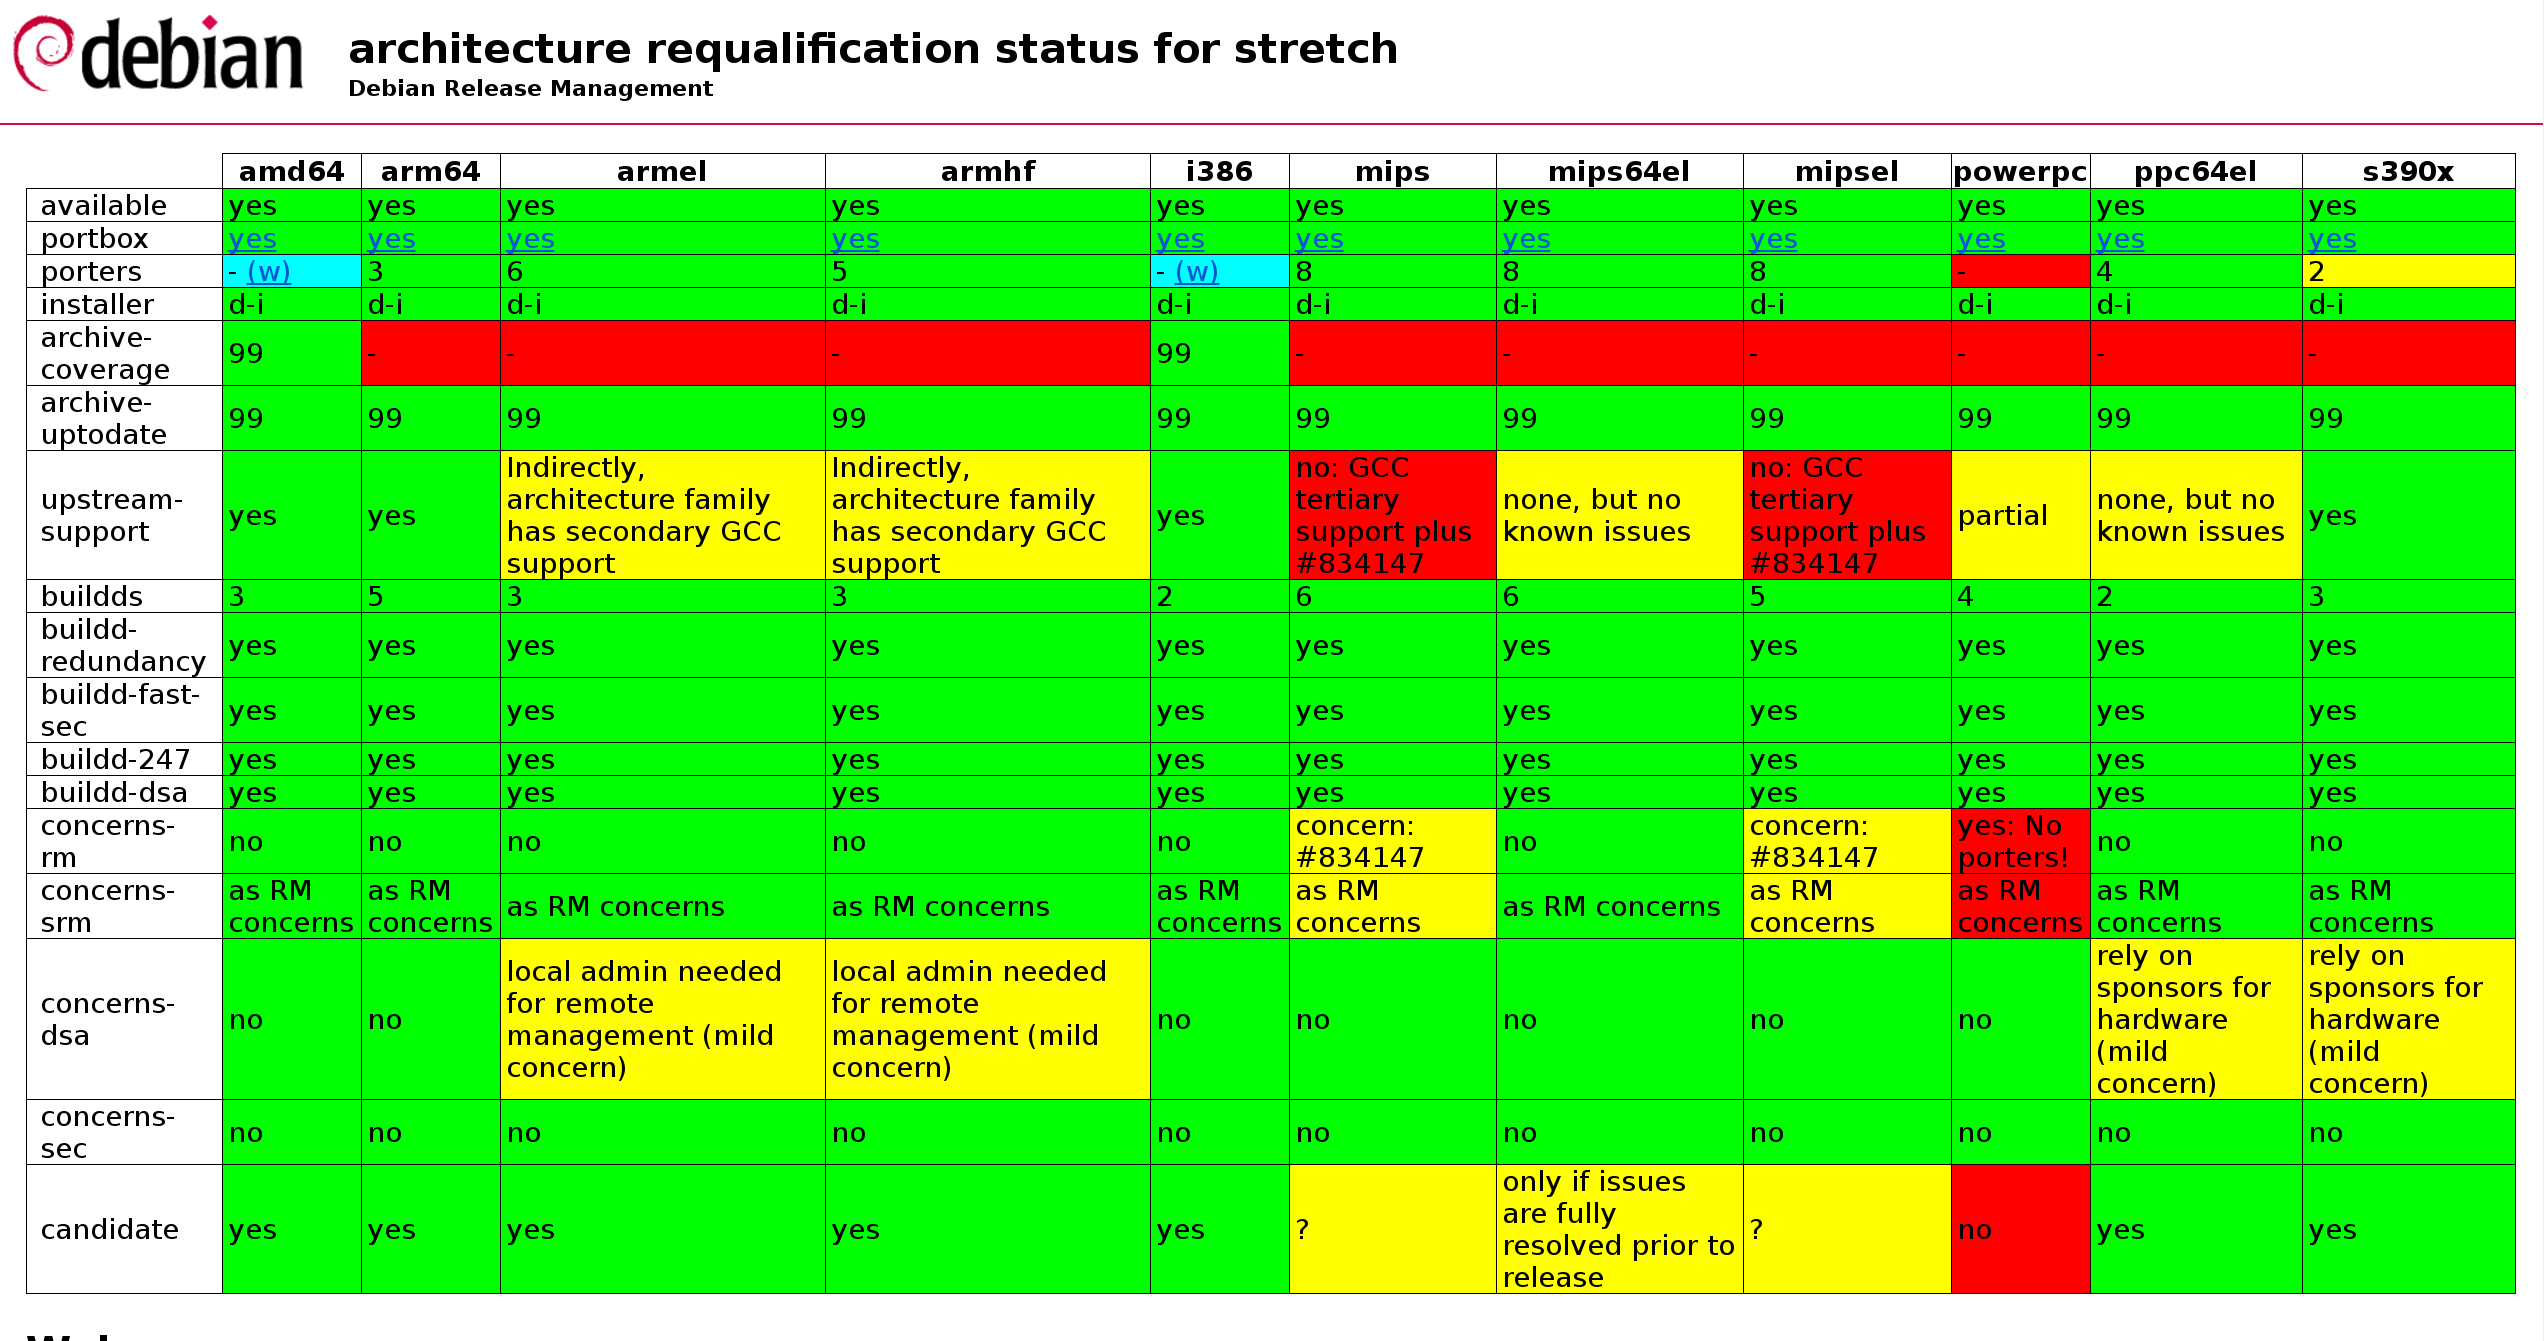
\includegraphics[width=.9\textwidth]{image201611/stretch-arch-requalification.png}
  \end{figure}
\end{frame}

\begin{frame}[c,fragile]{テーマ}
  \framesubtitle{- Next Debian Release -}
  \pause
  Soft waves by Juliette Taka Belin に決定。
  \begin{figure}
    \centering
    % https://wiki.debian.org/DebianArt/Themes/softWaves GPL-2+
    \includegraphics<2->[width=0.65\textwidth]{image201701/wallpaper.png}
  \end{figure}
\end{frame}

\begin{frame}[c,fragile]{Kernel, Software (予定)}
  \framesubtitle{- Next Debian Release -}
  \pause
  \begin{itemize}[<+->]
    \item%
      主なソフトウェア
      \begin{itemize}[<+->]
      \item[-] %
        Linux Kernel: \alert{4.10}
      \item[-] %
        GCC 6, binutils 2.27, glibc 2.22, LLVM 3.8, 3.9
      \item[-] %
        Perl 5.24.1, Python 2.7.11/3.5, Ruby 2.3 ,PHP 7.0.12, \\Go 1.7.3, OpenJDK 8
      \item[-] %
        GNOME 3.20, KDE 5.6.4, Xfce 4.12.3, lxde→lxqt 0.10?
      \item[-] %
        MySQL 5.6.30, MariaDB 10.0.28, PostgreSQL 9.6.1
        % , sqlite 3.15
      \item[-] %
        OpenSSL 1.1.0
      \item[-] %
        クロスコンパイラをデフォルトでサポートするように。
      \end{itemize}
    % \item%
    %   →アップデートが必要なパッケージがある場合は連絡ください。
  \end{itemize}
\end{frame}

\begin{frame}[c,fragile]{日本語によるDebianの情報}
  \framesubtitle{- Next Debian Release -}
  \begin{itemize}
  \item Debian JP Project
    \begin{itemize}
    \item[-]
      \url{http://www.debian.or.jp}
    \item[-]
      各種 ML、IRC channel 等も提供しています。
    \end{itemize}
  \item 東京エリアDebian勉強会
    \begin{itemize}
    \item[-]
      \url{http://tokyodebian.alioth.debian.org}
    \end{itemize}
  \item 関西エリアDebian勉強会
    \begin{itemize}
    \item[-]
      \url{https://wiki.debian.org/KansaiDebianMeeting}
    \end{itemize}
  \item Twitter: \url{@debian_jp}
  \end{itemize}
\end{frame}
\takahashi[60]{Have any Questions?}

\takahashi[60]{Thank you}

\takahashi[100]{ }

\end{document}
%%% Local Variables:
%%% mode: japanese-latex
%%% TeX-master: t
%%% End:
